%-----------------------------------------------------------------------------%
\chapter{LANDASAN TEORI}
%-----------------------------------------------------------------------------%

%
\vspace{4.5pt}

\section{Tinjauan Pustaka}
Pada bagian ini akan membahas teori-teori terkait yang digunakan pada penelitian ini.
\\

\subsection{Citra Digital}
Citra digital merupakan representasi dari fungsi intensitas cahaya dalam bentuk diskrit pada bidang dua dimensi. Citra tersusun oleh sekumpulan piksel (\textit{picture element}) yang memiliki koordinat (x,y) dan intensitas f(x,y). Koordinat (x,y) menunjukkan letak/posisi piksel dalam suatu citra, sedangkan intensitas f(x,y) menunjukkan nilai intensitas warna citra \cite{gonzalez}. Untuk membuat citra digital, diperlukan pengubahan data pengindraan kontinu menjadi bentuk digital. Tahap ini melibatkan dua proses, yaitu pengambilan sampel dan kuantisasi. Gambar \ref{img:CitraDigital} merupakan contoh dari citra digital.

\begin{table}[H]
	\small
	\begin{adjustbox}{width=1\textwidth}
		\begin{tabular}{| p {14cm} |}
			\hline
			\begin{figure}[H]
				\centering
				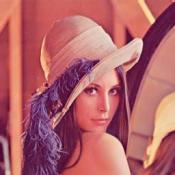
\includegraphics[width=7cm]{images/rgb.jpg}
			\end{figure} \\
			\hline
		\end{tabular}
	\end{adjustbox}
	\captionof{figure}{Contoh Citra Digital \cite{gonzalez}}
	\label{img:CitraDigital}
\end{table}

Suatu citra dapat bersifat kontinu sehubungan dengan koordinat x dan y, dan juga dalam intensitas. Untuk mengubahnya menjadi bentuk digital, harus dicoba fungsi dalam koordinat dan intensitas. \textit{Sampling} adalah proses untuk menentukan warna pada piksel tertentu pada citra dari sebuah gambar yang kontinu. Pada proses \textit{sampling} biasanya dicari warna rata-rata dari gambar analog yang kemudian dibulatkan. Proses \textit{sampling} sering juga disebut proses digitalisasi. \textit{Sampling} merupakan bagian dari metodologi statistika. Adakalanya, dalam proses \textit{sampling}, warna rata-rata yang didapat di relasikan ke level warna tertentu. Contohnya apabila dalam citra hanya terdapat 16 tingkatan warna abu-abu, maka nilai rata-rata yang didapat dari proses sampling harus diasosiasikan ke 16 tingkatan tersebut. Proses mengasosiasikan warna rata-rata dengan tingkatan warna tertentu disebut dengan kuantisasi.
\\ 

\subsection{Pengolahan Citra}
Pengolahan citra adalah salah satu cabang dari ilmu informatika (Komputer). Pengolahan citra berfokus pada usaha untuk melakukan transformasi suatu citra/gambar menjadi citra lain dengan menggunakan teknik tertentu. Berikut ini merupakan langkah-langkah yang umumnya dilakukan dalam merancang sebuah sistem pengolahan citra dan pengenalan pola:

\begin{table}[H]
	\small
	\begin{adjustbox}{width=1\textwidth}
		\begin{tabular}{| p {14cm} |}
			\hline
			\begin{figure}[H]
				\centering
				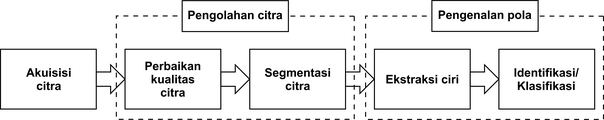
\includegraphics[width=14cm]{images/pencit}
			\end{figure} \\
			\hline
		\end{tabular}
	\end{adjustbox}
	\captionof{figure}{Proses Pengolahan Citra dan Pengenalan Pola}
	\label{img:pencit}
\end{table}

Operasi yang dilakukan untuk mengubah suatu citra menjadi citra lain dapat dikategorikan berdasarkan tujuan transformasi maupun cakupan operasi yang dilakukan terhadap citra. Berdasarkan tujuan transformasi operasi pengolahan citra dikategorikan menjadi peningkatan kualitas citra (\textit{Image Enhancement}) dan pemulihan citra (image restoration). Operasi peningkatan kualitas citra bertujuan untuk meningkatkan fitur tertentu pada citra. Sedangkan operasi pemulihan citra bertujuan untuk mengembalikan kondisi citra pada kondisi yang diketahui sebelumnya akibat adanya \textit{noise} yang menyebabkan penurunan kualitas citra. Berdasarkan cakupan operasi yang dilakukan terhadap citra, operasi pengolahan citra dikategorikan menjadi operasi titik, lokal, dan global. 

Operasi titik merupakan operasi yang dilakukan terhadap setiap piksel pada citra yang keluarannya hanya ditentukan oleh nilai piksel itu sendiri. Operasi titik dapat dibagi menjadi tiga macam, yaitu berdasarkan intensitas, geometri, dan gabungan keduanya. Contoh operasi titik berdasar intensitas adalah operasi pengambangan (\textit{thresholding}) yaitu membuat citra biner, operasi negatif (\textit{negative image}) yaitu membuat citra negatif, pemotongan citra (\textit{clipping}), dan pencerahan citra (\textit{image brightening}) yaitu menambahkan atau mengurangi konstanta untuk memperbaiki kecerahan pada citra. Operasi lokal merupakan operasi yang dilakukan terhadap setiap piksel pada citra yang keluarannya dipengaruhi oleh piksel tersebut dan piksel lainnya dalam suatu daerah tertentu. Salah satu contoh dari operasi berbasis lokal adalah operasi konvolusi untuk mendeteksi tepi (\textit{edge detection}) an pelembutan citra (\textit{image smoothing}). Operasi global merupakan operasi yang dilakukan tehadap setiap piksel pada citra yang keluarannya ditentukan oleh keseluruhan piksel yang membentuk citra. Contoh operasi global adalah operasi penyetaraan histogram untuk meningkatkan kualitas citra.\\

\subsection{\textit{Preprocessing}}
\textit{Preprocessing} merupakan proses pengolahan data asli sebelum tahapan pengolahan data. Proses ini bertujuan agar data siap untuk diproses ke tahap ektraksi fitur. Preprocessing memiliki tujuan untuk menghilangkan derau, memperjelas fitur, mengubah ukuran citra, dan konversi data. Contoh dari \textit{preprocessing} yaitu pengabuan citra (\textit{grayscaling}), binerisasi citra, \textit{croping} citra, dan \textit{resize} citra \cite{gonzalez}.\\ 

\subsubsection{Pengabuan Citra}
Citra \textit{grayscale} adalah suatu citra yang hanya memiliki warna berupa tingkat keabuan. Citra \textit{grayscale} digunakan karena membutuhkan sedikit informasi yang diberikan pada tiap piksel dibandingkan dengan citra berwarna sehingga dalam \textit{grayscale} image hanya membutuhkan nilai intensitas tunggal dibandingkan dengan citra berwarna membutuhkan tiga intensitas untuk tiap pikselnya. Intensitas dari citra \textit{grayscale} disimpan dalam 8 bit integer yang memberikan 256 kemungkinan yang mana dimulai dari level 0 sampai dengan 255 (0 untuk hitam dan 255 untuk putih) \cite{gonzalez}. Gambar \ref{img:grayscale} merupakan contoh dari citra \textit{grayscale}.

\begin{table}[H]
	\small
	\begin{adjustbox}{width=1\textwidth}
		\begin{tabular}{| p {14cm} |}
			\hline
			\begin{figure}[H]
				\centering
				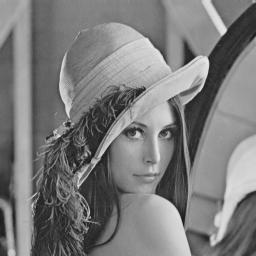
\includegraphics[width=7cm]{images/grayscale.jpg}
			\end{figure} \\
			\hline
		\end{tabular}
	\end{adjustbox}
	\captionof{figure}{Contoh Citra \textit{Grayscale} \cite{gonzalez}}
	\label{img:grayscale}
\end{table}

Persamaan pengabuan citra dapat dilihat pada persamaan \ref{eq:grayscale} dengan \textit{R} melambangkan intensitas warna merah, \textit{G} untuk intensitas warna hijau, dan \textit{B} untuk intensitas warna biru. 

\begin{table}[H]
	\begin{adjustbox}{width=1\textwidth}
		\begin{tabular}{|p{13.55cm}|}
			\hline
			\begin{equation}
			Gray value = 0.299 R + 0.587 G + 0.114 B
			\label{eq:grayscale}
			\end{equation}\\
			\hline
		\end{tabular}
	\end{adjustbox}
\end{table}

Persamaan \ref{eq:grayscale} menyimpulkan bahwa persentase warna hijau yang paling besar karena manusia cenderung lebih sensitif terhadap perubahan warna hijau yang memiliki panjang gelombang sekitar 500-570 nm, merah, lalu biru, dan merupakan rekomendasi dari \textit{International Telecommunication Union Radiocommunication Sector}.\\

\subsubsection{Citra Biner}
Citra biner (\textit{binary image}) adalah citra yang hanya mempunyai dua nilai derajat keabuan yaitu hitam dan putih. Citra biner bernilai 1 untuk objek dan 0 untuk latar belakang. Citra biner sering kali digunakan karena mempercepat waktu proses dan memperkecil penggunaan memori\cite{munir}. Meskipun komputer saat ini dapat memproses citra hitam-putih (\textit{grayscale}) maupun citra berwarna, namun citra biner masih tetap dipertahankan keberadaannya. 

\begin{table}[H]
	\small
	\begin{adjustbox}{width=1\textwidth}
		\begin{tabular}{| p {14cm} |}
			\hline
			\begin{figure}[H]
				\centering
				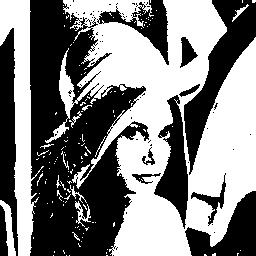
\includegraphics[width=7cm]{images/biner.jpg}
			\end{figure} \\
			\hline
		\end{tabular}
	\end{adjustbox}
	\captionof{figure}{Contoh Citra Biner \cite{gonzalez}.}
	\label{img:binary}
\end{table}

Sama seperti citra \textit{grayscale}, citra biner juga merupakan citra yang hanya memiliki satu kanal warna. Citra biner memiliki kedalaman bit sebesar 1-bit. \textit{Thresholding} adalah metode untuk mengubah citra \textit{grayscale} menjadi citra biner sehingga objek dapat dipisahkan dari \textit{background}. Untuk mendapat nilai \textit{threshold} yang adaptif menggunakan metode Otsu. Nilai intensitas warna pada setiap piksel citra biner dibagi menjadi 2$\land$1 = 2 warna yaitu warna hitam yang dinyatakan oleh nilai 0 dan warna putih yang dinyatakan oleh nilai 1. Persamaan yang digunakan untuk mengkonversi nilai piksel citra \textit{grayscale} menjadi biner pada metode \textit{thresholding} adalah:

\begin{table}[H]
	\small
	\begin{adjustbox}{width=1\textwidth}
		\begin{tabular}{|p{13.55cm}|}
			\hline
			\begin{equation} \label{eqn:biner}
			\displaystyle
			g(x,y) = \left\{\begin{array}{l}1, jika f(x,y) \ge T \\0, jika f(x,y) < T\end{array}\right.
			\end{equation} \\
			\hline
		\end{tabular}
	\end{adjustbox}
\end{table}

\noindent
\renewcommand{\arraystretch}{1}
\begin{tabularx}{\textwidth}{lll}
	\hline
	Keterangan: \\
	$g(x,y)$ & : & citra biner\\
	$f(x,y)$ & : & citra \textit{grayscale}\\
	$T$ & : & \textit{treshold}\\
	\hline
\end{tabularx}
\vspace{4.5pt} 

Citra biner digunakan saat proses penentuan ROI. ROI yang berupa citra biner digunakan untuk menandai lokasi dimana mobil akan melaju. ROI yang digunakan berupa template dari dataset yang diperoleh.\\

\subsubsection{\textit{Otsu Tresholding}}
Tujuan dari metode Otsu adalah membagi histogram citra gray level kedalam dua daerah yang berbeda secara otomatis tanpa membutuhkan bantuan pengguna untuk memasukkan nilai ambang. Pendekatan yang dilakukan oleh metode otsu adalah dengan melakukan analisis diskriminan yaitu menentukan suatu variabel (nilai ambang atau \textit{threshold}) yang dapat membedakan antara dua atau lebih kelompok yang muncul secara alami. Analisis Diskriminan akan memaksimumkan nilai ambang agar dapat membagi objek latar depan (\textit{foreground}) dan latar belakang (\textit{background}).

Langkah  awal  yang harus  dilakukan  adalah  membuat  histogram.  Dari histogram dapat diketahui jumlah piksel untuk setiap tingkat  keabuan.  Tingkat  keabuan  citra  dinyatakan dengan i sampai dengan L. Level ke i dimulai dari 1, yaitu  piksel  0.  Untuk L,  maksimal  level  adalah  256 dengan piksel bernilai 255. Nilai  ambang  yang  akan  dicari  dari  suatu  citra \textit{grayscale} dinyatakan dengan k. Nilai kberkisar antara 0  sampai  dengan L - 1,  dengan  nilai L = 256  (simbol histogram adalah Pi) \cite{otsu}. Jadi probabilitas setip piksel pada level ke i dinyatakan dengan persamaan berikut. 

\begin{table}[H]
	\small
	\begin{adjustbox}{width=1\textwidth}
		\begin{tabular}{|p{13.55cm}|}
			\hline
			\begin{equation} \label{eqn:otsu1}
			\displaystyle
			P_{i} = \frac{n_{i}}{N}
			\end{equation} \\
			\hline
		\end{tabular}
	\end{adjustbox}
\end{table}

\noindent
\renewcommand{\arraystretch}{1}
\begin{tabularx}{\textwidth}{lll}
	\hline
	Keterangan: \\
	$P_{i}$ & : & probabilitas piksel ke-i\\
	$n_{i}$ & : & jumlah piksel dengan tingkat keabuan i\\
	$N$ & : & total jumlah piksel pada citra\\
	\hline
\end{tabularx}
\vspace{4.5pt}

Langkah   selanjutnya   mencari   nilai   jumlah kumulatif, rerata  kumulatif  dan  intensitas  global. mencari  nilai  tersebut  dapat  melihat  persamaan  \eqref{eqn:otsu2}, persamaan \eqref{eqn:otsu3}, dan persamaan \eqref{eqn:otsu4}.

\begin{table}[H]
	\small
	\begin{adjustbox}{width=1\textwidth}
		\begin{tabular}{|p{13.55cm}|}
			\hline
			\begin{equation} \label{eqn:otsu2}
			\displaystyle
			\omega (k) = \sum\limits_{i=0}^{k} p_{i}
			\end{equation} 
			
			\begin{equation} \label{eqn:otsu3}
			\displaystyle
			\mu (k) = \sum\limits_{i=0}^{k} i . p_{i}
			\end{equation}
			 
			\begin{equation} \label{eqn:otsu4}
			\displaystyle
			\mu _{T} (k) = \sum\limits_{i=0}^{L-1} i . p_{i}
			\end{equation}\\
			\hline
		\end{tabular}
	\end{adjustbox}
\end{table}

\noindent
\renewcommand{\arraystretch}{1}
\begin{tabularx}{\textwidth}{lll}
	\hline
	Keterangan: \\
	$k$ & : &  tingkat level keabuan  dimana  setiap  rentang  piksel  akan  dihitung\\
	$\omega (k)$ & : & jumlah kumulatif\\
	$\mu (k)$ & : & rerata Kumulatif\\
	$\mu _{T} (k)$ & : & rerata Intensitas Global\\
	\hline
\end{tabularx}
\vspace{4.5pt}

Langkah selanjutnya adalah menentukan varian antar kelas  (\textit{between class variance}).

\begin{table}[H]
	\small
	\begin{adjustbox}{width=1\textwidth}
		\begin{tabular}{|p{13.55cm}|}
			\hline
			\begin{equation} \label{eqn:otsu5}
			\displaystyle
			\sigma_{B}^{2} (k)  = \frac{[\mu _{T}\omega (k)-\mu (k)] ^2}{\omega (k)[1 - \omega (k)]}
			\end{equation} \\
			\hline
		\end{tabular}
	\end{adjustbox}
\end{table}

\noindent
\renewcommand{\arraystretch}{1}
\begin{tabularx}{\textwidth}{lll}
	\hline
	Keterangan: \\
	$\sigma_{B}^{2}$ & : & nilai ambang\\
	$k$ & : &  tingkat level keabuan  dimana  setiap  rentang  piksel  akan  dihitung\\
	$\omega (k)$ & : & jumlah kumulatif\\
	$\mu (k)$ & : & rerata Kumulatif\\
	$\mu _{T} (k)$ & : & rerata Intensitas Global\\
	\hline
\end{tabularx}
\vspace{4.5pt}

Hasil  dari  perhitungan \textit{between class variance} dicari   nilai   maksimal.   Nilai   yang   paling   besar digunakan  sebagai \textit{threshold} atau  nilai  ambang  (k), dengan persamaan \eqref{eqn:otsu6}.

\begin{table}[H]
	\small
	\begin{adjustbox}{width=1\textwidth}
		\begin{tabular}{|p{13.55cm}|}
			\hline
			\begin{equation} \label{eqn:otsu6}
			\displaystyle
			\sigma_{B}^{2} (k\star)  = max_{1 \leq x \leq L} \sigma_{B}^{2}
			\end{equation} \\
			\hline
		\end{tabular}
	\end{adjustbox}
\end{table}

\noindent
\renewcommand{\arraystretch}{1}
\begin{tabularx}{\textwidth}{lll}
	\hline
	Keterangan: \\
	$\sigma_{B}^{2}$ & : & nilai ambang maksimal\\
	$\omega (k)$ & : & jumlah kumulatif\\
	$\mu (k)$ & : & rerata Kumulatif\\
	$\mu _{T} (k)$ & : & rerata Intensitas Global\\
	$\sigma_{B}^{2}$ & : & nilai ambang\\
	$k$ & : &  tingkat level keabuan  dimana  setiap  rentang  piksel  akan  dihitung\\
	\hline
\end{tabularx}
\vspace{4.5pt}

\textit{Between class variance} bertujuan untuk mencari nilai   ambang dari sebuah citra \textit{grayscale}, nilai ambang atau \textit{threshold} digunakan sebagai nilai acuan untuk mengubah citra \textit{grayscale} ke citra biner. Setiap citra memiliki nilai ambang yang berbeda-beda.
\\

\subsubsection{Derau}
Derau (\textit{Noise}) merupakan piksel yang mengganggu kualitas citra. Derau dapat disebabkan oleh gangguan fisis (optik) pada alat akuisisi maupun secara disengaja akibat proses pengolahan yang tidak sesuai \cite{gonzalez}. Beberapa gangguan mungkin saja terjadi saat pengambilan citra, seperti kamera tidak fokus atau munculnya bintik-bintik yang bisa terjadi karena proses pengambilan gambar yang tidak sempurna. Setiap gangguan pada citra dinamakan derau, yang tidak hanya terjadi karena ketidak sempurnaan dalam proses pengambilan citra, tetapi dapat disebabkan juga oleh noda kotoran yang terjadi pada citra setelah pengambilan citra. Contohnya adalah bintik hitam atau putih yang muncul secara acak yang tidak diinginkan di dalam citra. Bintik acak ini disebut dengan derau \textit{salt and pepper}. \textit{Salt and Pepper} merupakan \textit{noise} yang terkadang muncul pada citra. \textit{Noise} ini dapat terjadi karena adanya gangguan pada citra, misalnya temperatur. \textit{Salt and Pepper} pada citra berupa piksel hitam putih yagn tersebar seperti pada gambar \ref{fig:ContohDerau}.

\begin{table}[H]
	\small
	\begin{adjustbox}{width=1\textwidth}
		\begin{tabular}{| p {14cm} |}
			\hline
			\begin{figure}[H]
				\centering
				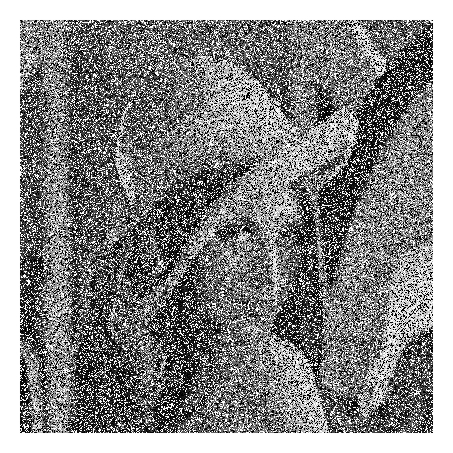
\includegraphics[width=7cm]{images/noise_snp}
			\end{figure} \\
			\hline
		\end{tabular}
	\end{adjustbox}
	\captionof{figure}{Contoh Derau \textit{Salt and Pepper} \cite{gonzalez}.}
	\label{fig:ContohDerau}
\end{table}

\subsubsection{Segmentasi Citra}
Segmentasi citra adalah membagi suatu citra menjadi wilayah - wilayah yang homogen \cite{gonzalez}. Tahapan ini bertujuan untuk mempartisi citra menjadi bagian-bagian pokok yang mengandung informasi penting. Misalnya, memisahkan objek dan latar belakang. Segmentasi terdiri dari \textit{downsampling}, penipisan dan deteksi tepian. 

Tahap \textit{downsampling} merupakan proses untuk menurunkan jumlah piksel dan menghilangkan sebagian informasi dari citra. Dengan resolusi citra yang tetap, downsampling menghasilkan ukuran citra yang lebih kecil. \textit{Thinning} (penipisan) adalah proses mengurangi suatu obyek didalam citra digital menjadi ukuran yang minimum (objek (\textit{region}) direduksi menjadi rangka (\textit{skeleton})). \textit{Thinning} hanya digunakan pada citra biner dan menghasilkan citra biner lain sebagai outputnya . \textit{Thinning} bertujuan untuk mengurangi bagian yang tidak perlu (\textit{redudant}) sehingga hanya dihasilkan informasi yang penting saja. Pola hasil penipisan harus tetap menyerupai bentuk pola asal. Penentuan tepian suatu objek dalam citra merupakan salah satu wilayah pengolahan citra digital yang paling awal dan paling banyak diteliti. Proses ini seringkali ditempatkan sebagai langkah pertama dalam aplikasi segmentasi citra, yang bertujuan untuk mengenali objek-objek yang terdapat dalam citra ataupun konteks citra secara keseluruhan. Deteksi tepi berfungsi untuk mengidentifikasi garis batas (\textit{boundary}) dari suatu objek yang terdapat pada citra.

Algoritme segmentasi didasarkan pada 2 buah karakteristik nilai derajat kecerahan citra, yaitu: \textit{discontinuity} dan \textit{similarity}. Pada \textit{discontinuity}, citra dipisahkan/dibagi atas dasar perubahan yang mencolok dari derajad kecerahannya. Aplikasi yang umum adalah untuk deteksi titik, garis, area, dan sisi citra. Pada \textit{similarity} didasarkan atas \textit{thresholding, region growing}, dan \textit{region spiltting and merging}.
\\

\subsubsection{Deteksi Tepi}
Deteksi tepi (\textit{Edge detection}) adalah operasi yang dijalankan untuk mendeteksi garis tepi (\textit{edges}) yang membatasi dua wilayah citra homogen yang memiliki tingkat kecerahan yang berbeda \cite{gonzalez}. Tujuannya adalah untuk mengubah citra 2D menjadi bentuk kurva. Metode yang banyak digunakan untuk proses deteksi tepi adalah metode Robert, Prewitt, Sobel, dan Canny. Hasil dari metode - metode deteksi tepi dapat dilihat pada gambar \ref{fig:ContohDeteksiTepi}.

\begin{table}[H]
	\small
	\begin{adjustbox}{width=1\textwidth}
		\begin{tabular}{| p {14cm} |}
			\hline
			\begin{figure}[H]
				\centering
				\subfloat[ ]{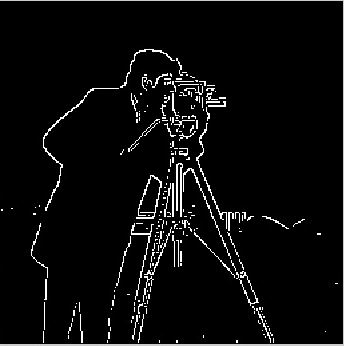
\includegraphics[width = 5cm]{images/roberts}} 
				\subfloat[ ]{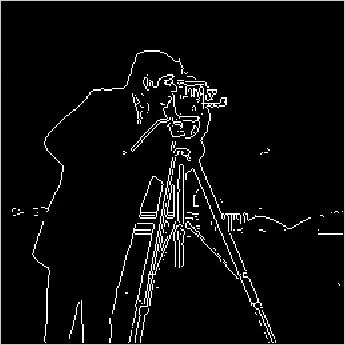
\includegraphics[width = 5cm]{images/prewitt}}\\
				\subfloat[ ]{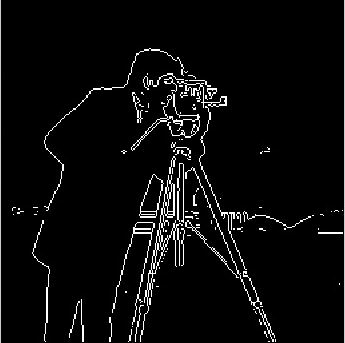
\includegraphics[width = 5cm]{images/sobel}}
				\subfloat[ ]{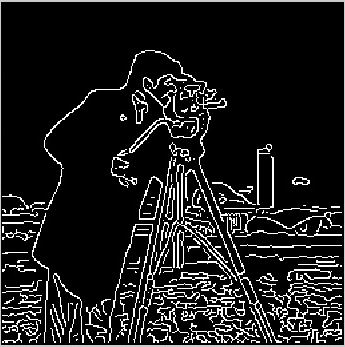
\includegraphics[width = 5cm]{images/canny}} 
			\end{figure} \\
			\hline
		\end{tabular}
	\end{adjustbox}
	\captionof{figure}{Contoh Deteksi Tepi \cite{gonzalez}. (a) Robert (b) Prewitt (c) Sobel (d) Canny}
	\label{fig:ContohDeteksiTepi}
\end{table}

Metode pada deteksi tepi terletak pada penggunaan kernel yang berbeda. Metode Sobel merupakan pengembangan metode robert dengan menggunakan filter HPF yang diberi satu angka nol penyangga. Metode ini mengambil prinsip dari fungsi laplacian dan gaussian yang dikenal sebagai fungsi untuk membangkitkan HPF. Kelebihan dari metode sobel ini adalah kemampuan untuk mengurangi noise sebelum melakukan perhitungan deteksi tepi. Kernel filter yang digunakan dalam metode Sobel ini adalah: 

\begin{center}
	\begin{tabular}{ c c c}
		$
		x = 
		\left[ \begin{array}{rcl}
		-1 & -2 & -1 \\ 
		0 & 0 & 0 \\
		1 & 2 & 1 \end{array} \right]
		\mbox{~dan~}
		y =
		\left[ \begin{array}{rcl}
		-1 & 0 & 1 \\ 
		-2 & 0 & 2 \\
		-1 & 0 & 1 \end{array} \right]
		$
	\end{tabular}
\end{center}

%Kemudian kernel untuk deteksi garis diagonal menggunakan:

%\begin{center}
%	\begin{tabular}{ c c c}
%		$
%		X = 
%		\left[ \begin{array}{rcl}
%		-0 & 1 & 2 \\ 
%		-1 & 0 & 1 \\
%		-2 & -1 & 0 \end{array} \right]
%		\mbox{~dan~}
%		Y =
%		\left[ \begin{array}{rcl}
%		-2 & -1 & 0 \\ 
%		-1 & 0 & 1 \\
%		0 & 1 & 2 \end{array} \right]
%		$
%	\end{tabular}
%\end{center}

Koordinat x didefinisikan di sini sebagai peningkatan pada arah horizontal, dan koordinat y didefinisikan sebagai peningkatan pada arah vertikal. Pada setiap titik dalam gambar, perkiraan gradien yang dihasilkan dapat dikombinasikan untuk memberikan besarnya gradien menggunakan rumus:

\begin{table}[H]
	\small
	\begin{adjustbox}{width=1\textwidth}
		\begin{tabular}{|p{13.55cm}|}
			\hline
			\begin{equation} \label{eqn:sobel}
			\displaystyle
			|G| = \sqrt{G_{x}^{2}+G_{y}^{2}}
			\end{equation} \\
			\hline
		\end{tabular}
	\end{adjustbox}
\end{table}

\noindent
\renewcommand{\arraystretch}{1}
\begin{tabularx}{\textwidth}{lll}
	\hline
	Keterangan: \\
	$G$ & : & gradien\\
	$G_{x}$ & : & arah sumbu X\\
	$G_{y}$ & : & arah sumbu Y\\
	\hline
\end{tabularx}
\vspace{4.5pt}

\subsubsection{\textit{Region of Interest} (ROI)}
\textit{Region   of  Interest}   adalah  suatu   bagian   dari   citra   yang   dipilih   untuk kemudian  diproses. Daerah  tersebut  dibedakan  dengan  menggunakan klasifikasi dan \textit{masking}.  Jika  piksel pada   \textit{mask}  tidak   nol,   maka   pemrosesan   citra   dilakukan. Sebaliknya jika piksel pada \textit{mask} sama dengan nol, proses tidak dijalankan. Setelah  daerah yang diinginkan ditemukan, daerah  tersebut  ditandai dengun kotak  untuk  membatasi  daerah  yang akan  dikenali. Dalam  \textit{Region  of  Interest}, citra  dapat  didefinisikan lebih  dari  satu  region (bagian). \textit{Region  of Interest}  sangat membantu untuk  segmentasi dalam  pemrosesan citra karena  dengan  menggunakan teknik  ini  citra  atau  obyek  dapat  lebih mudah dikenali. Karena obyek sudah akan dibagi dalam \textit{region - region} tertentu  sesuai dengan citra obyeknya. \textit{Region  of  Interest} membantu dalam mengurangi penggunaan memori.\\

\subsubsection{\textit{Sliding Window}}
Pada bidang \textit{computer vision}, \textit{sliding window} merupakan sebuah daerah persegi atau persegi panjang yang memiliki ukuran tertentu dan akan bergeser dengan jarak tertentu secara berurutan ke seluruh daerah citra. Tahap ini dilakukan untuk memproses citra lokal secara bergantian dan pada umumnya digunakan untuk prooses pencarian dari suatu citra. Ukuran dari \textit{window} dan jarak perpindahan antar \textit{window} yang digunakan tergantung dari masalah yang akan diselesaikan maka biasanya ukuran tersebut disesuaikan dengan ukuran objek pada citra. Ukuran \textit{window} yang optimal adalah \textit{window} yang dapat mencakup keseluruhan objek, tidak terlalu besar atau kecil, oleh karena itu, perlu dilakukan alanilis objek citra agar mendapatkan keseluruhan objek. Sama halnya dengan jarak perpindahan antar \textit{window}, bila terlalu besar akan terdapat bagian citra yagn terlewat, bila terlalu kecil akan menyebabkan waktu komputasi yang lebih lama. 

\subsection{Ekstraksi Fitur}
Ekstraksi fitur merupakan suatu pengambilan ciri (fitur) dari suatu bentuk yang nantinya nilai yang didapatkan akan dianalisis untuk proses selanjutnya \cite{gonzalez}. Ekstraksi fitur bertujuan untuk mencari daerah fitur yang signifikan pada gambar. Ekstraksi fitur dilakukan dengan cara menghitung jumlah titik atau piksel yang ditemui dalam setiap pengecekan, dimana pengecekan dilakukan dalam berbagai arah pengecekan pada koordinat kartesian dari citra digital yang dianalisis, yaitu vertikal, horizontal. Ciri yang telah diekstrak kemudian digunakan sebagai parameter / nilai masukan untuk membedakan antara objek satu dengan lainnya pada tahapan identifikasi/ klasifikasi. Ekstraksi fitur terbagi menjadi tiga macam yaitu ekstraksi fitur bentuk, ekstraksi fitur tekstur, ekstraksi fitur warna.

Bentuk dari suatu objek adalah karakter permukaan yang diwakili oleh garis dan kontur. Fitur bentuk dikategorikan bergantung pada teknik yang digunakan berdasarkan daerah (\textit{region-based}) dan berdasarkan batas (\textit{boundary-based}). Teknik berdasarkan daerah (\textit{region-based}) menggambarkan bentuk wilayah dengan menggunakan karakteristik internal, contohnya adalah piksel yang berada dalam suatu wilayah. Sedangkan teknik berdasarkan batas (\textit{boundary-based}) menggambarkan bentuk daerah dengan menggunakan karakteristik eksternal, contohnya adalah piksel sepanjang batas objek.

Pada ekstraksi fitur tekstur, fitur pembeda adalah tekstur yang merupakan karakteristik penentu pada citra. Teknik statistik yang terkenal untuk ekstraksi fitur adalah matriks gray level co-occurrence. Teknik tersebut dilakukan dengan melakukan pemindaian untuk mencari jejak derajat keabuan setiap dua buah piksel yang dipisahkan dengan jarak d dan sudut $\theta$ yang tetap. Biasanya sudut yang digunakan adalah 0, 45, 90, dan 135. Sedangkan pada ekstraksi fitur warna, ciri pembeda adalah warna. Biasanya ekstraksi fitur ini digunakan pada citra berwarna yang memiliki komposisi warna RGB (red, green, blue).
\\

\subsubsection{\textit{Histogram of Oriented Gradients}}
\textit{Histogram of Oriented Gradients} (HOG) merupakan metode ekstraksi fitur bentuk berupa garis dengan memperhatikan distribusi gradien intensitas lokal atau arah tepi. Dalam praktiknya ini dilakukan dengan membagi jendela gambar menjadi wilayah spasial kecil ("sel"). Untuk setiap sel mengumpulkan histogram 1-D lokal dari arah gradien atau orientasi tepi atas piksel sel. Sel dikumpulkan menjadi blok untuk dinormalisasi. Blok deskriptor hasil normalisasi disebut deskriptor HOG \cite{dalal}. Pertama akan dihitung gradien untuk setiap piksel pada citra dari sumbu x dan y dengan menggunakan : 

\begin{table}[H]
	\small
	\begin{adjustbox}{width=1\textwidth}
		\begin{tabular}{|p{13.55cm}|}
			\hline
			\begin{equation} \label{eqn:GradientH}
			\displaystyle
			G_{x}(x,y) = I(x+1,y) - I(x-1,y)
			\end{equation} 
			
			\begin{equation} \label{eqn:GradientV}
			\displaystyle
			G_{y}(x,y) = I(x,y+1) - I(x,y-1)
			\end{equation}\\
			\hline
		\end{tabular}
	\end{adjustbox}
\end{table}

\noindent
\renewcommand{\arraystretch}{1}
\begin{tabularx}{\textwidth}{lll}
	\hline
	Keterangan: \\
	$G_{x}(x,y)$ & : & gradien sumbu x\\
	$G_{y}(x,y)$ & : & gradien sumbu y\\
	$I(x,y)$ & : & nilai piksel citra dari baris x dan dan kolom y\\
	\hline
\end{tabularx}
\vspace{4.5pt}

Setelah mendapat gradien dari sumbu x dan y dari setiap piksel, besar nilai dan arah gradien dihitung menggunakan:
\begin{table}[H]
	\small
	\begin{adjustbox}{width=1\textwidth}
		\begin{tabular}{|p{13.55cm}|}
			\hline
			\begin{equation} \label{eqn:BesarGradien}
			\displaystyle
			G(x,y) = \sqrt{G_{x}(x,y)^{2}+G_{y}(x,y)^{2}}
			\end{equation} 
			
			\begin{equation} \label{eqn:ArahGradien}
			\displaystyle
			\theta(x,y) = \arctan\frac{G_{y}(x,y)}{G_{x}(x,y)}
			\end{equation}\\
			\hline
		\end{tabular}
	\end{adjustbox}
\end{table}

\noindent
\renewcommand{\arraystretch}{1}
\begin{tabularx}{\textwidth}{lll}
	\hline
	Keterangan: \\
	$G(x,y)$ & : & besar nilai gradien sumbu x dan y\\
	$\theta(x,y)$ & : & arah nilai gradien sumbu x dan y\\
	\hline
\end{tabularx}
\vspace{4.5pt}

Setiap piksel pada citra kemudian dibagi ke dalam sel, yang kemudian dihitung persebaran HOGnya menggunakan vote. Pertama, proses vote pada HOG dilakukan dengan membagi jumlah sudut gradien ke dalam jumlah \textit{orientation bin} untuk menentukan nilai - nilai dari \textit{bin}. Untuk setiap arah sudut gradien dari setiap piksel dalam sel dimasukkan ke dalam rentang \textit{orientation bin} yang sudah ditentukan. Besar nilai gradien kemudian dibagi dengan \textit{orientation bin} yang berhubungan. HOG dibuat untuk setiap sel.

Selanjutnya dilakukan normalisasi terhadap vote pada setiap \textit{bin} dalam sel. Normalisasi dilakukan dalam 1 blok dengan ukuran m x n sel. Metode untuk normalisasi terdapat sebanyak 4 buah meliputi: \textit{L2-Norm, L2-Hys, L1-sqrt, dan L1-norm}. Pada penelitian ini, akan digunakan normalisasi dengan metode \textit{L2-Norm} dengan persamaan:

\begin{table}[H]
	\small
	\begin{adjustbox}{width=1\textwidth}
		\begin{tabular}{|p{13.55cm}|}
			\hline
			\begin{equation} \label{eqn:normalisasi2}
			\displaystyle
			f =\sqrt{ \frac{v}{\sum\limits_{n=1}^{N} v}}
			\end{equation} \\
			\hline
		\end{tabular}
	\end{adjustbox}
\end{table}

\noindent
\renewcommand{\arraystretch}{1}
\begin{tabularx}{\textwidth}{lll}
	\hline
	Keterangan: \\
	$v$ & : & bobot vektor hasil \textit{L1-Sqrt} yang mewakili setiap \textit{bin}\\
	$i$ & : & nilai counter i sampai dengan N\\
	$N$ & : & total nilai \textit{bin} untuk normalisasi\\
	\hline
\end{tabularx}
\vspace{4.5pt}

Untuk algoritme rumus normalisasi L2-Hys merupakan algoritma mengikuti dari L2-Norm, namun dengan membatasi nilai maksimal hasil normalisasi sebesar 0,2.

Proses normalisasi blok dilakukan dengan sliding window yang melakukan proses dengan pergeseran sebesar 1x ukuran sel secara vertikal dan horizontal. Proses ini akan bersifat overlapping untuk beberapa sel yang dinormalisasi sehingga menimbulkan informasi yang redundan, namun akurasi yang dihasilkan justru semakin meningkat \cite{opencv}.
\\

\subsection{Klasifikasi}
Klasifikasi adalah sebuah proses untuk menemukan sebuah model yang menjelaskan dan membedakan konsep atau kelas data dengan tujuan memperkirakan kelas dari suatu objek yang kelasnya tidak diketahui \cite{steinwart}. 
\\ 

\subsubsection{\textit{Support Vector Machine}}
\textit{Support Vector Machines} (SVM) merupakan metode klasifikasi. SVM mengelompokkan fitur menjadi beberapa kelas menggunakan \textit{hyperplane} pada suatu ruang yang disebut \textit{feature space}.

\begin{table}[H]
	\small
	\begin{adjustbox}{width=1\textwidth}
		\begin{tabular}{| p {14cm} |}
			\hline
			\begin{figure}[H]
				\centering
				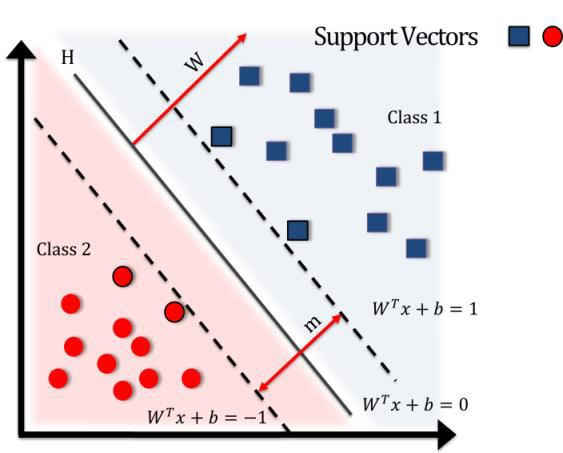
\includegraphics[width=6cm]{images/svm.jpg}
			\end{figure} \\
			\hline
		\end{tabular}
	\end{adjustbox}
	\captionof{figure}{Contoh \textit{Hyperplane} pada SVM \cite{bougharriou}.}
	\label{img:hyerplane_svm}
\end{table}
Berdasarkan contoh pada gambar \ref{img:hyerplane_svm}, \textit{hyperplane} merupakan sebuah indikator pemisah dimana ditentukan berdasarkan \textit{training} dengan margin tertinggi \cite{steinwart}. \textit{Hyperplane} yang optimal harus memenuhi persamaan berikut:
\begin{table}[H]
	\small
	\begin{adjustbox}{width=1\textwidth}
		\begin{tabular}{|p{13.55cm}|}
			\hline
			\begin{equation} 
			\label{eqn:hiperplane}
			w^T \cdot x + b = 0
			\end{equation}\\
			\hline
		\end{tabular}
	\end{adjustbox}
\end{table}

\noindent
\renewcommand{\arraystretch}{1}
\begin{tabularx}{\textwidth}{lll}
\hline
Keterangan: \\
$w$ & : & vektor berat\\
$.$ & : & perkalian vektor\\
$x$ & : & vektor input\\
$b$ & : & nilai bias\\
\hline
\end{tabularx}
\vspace{4.5pt}

Proses pemetaan dalam SVM menggunakan kernel, dan kernel yang biasanya digunakan adalah RBF (\textit{Radiant Basis Function}). Berikut rumus kernel RBF:
\begin{table}[H]
	\small
	\begin{adjustbox}{width=1\textwidth}
		\begin{tabular}{|p{13.55cm}|}
			\hline
			\begin{equation} 
			\label{eqn:jarakfitur}
			K(x,z) = e^{-((x-z)^2/(2\sigma^2)}
			\end{equation}\\
			\hline
		\end{tabular}
	\end{adjustbox}
\end{table}

\noindent
\renewcommand{\arraystretch}{1}
\begin{tabularx}{\textwidth}{lll}
	\hline
	Keterangan: \\
	$x  dan  z$ & : & pasangan dua data training\\
	$\sigma$ & : & konstanta\\
	\hline
\end{tabularx}
\vspace{4.5pt}

Klasifikasi non-linier dilakukan menggunakan persamaan:
\begin{table}[H]
	\small
	\begin{adjustbox}{width=1\textwidth}
		\begin{tabular}{|p{13.55cm}|}
			\hline
			\begin{equation}
			\label{eqn:rbfkernel} 
			f(x) = sign(\sum\limits_{i=1}^{m}\alpha_{i}y_{i}K()x,x_{i}+b)
			\end{equation}\\
			\hline
		\end{tabular}
	\end{adjustbox}
\end{table}

\noindent
\renewcommand{\arraystretch}{1}
\begin{tabularx}{\textwidth}{lll}
	\hline
	Keterangan: \\
	$\alpha_{i}$ & : & alpha\\
	$y_{i}$ & : & kelas\\
	$K(x,x_{i})$ & : & kernel matriks\\
	$b$ & : & bias\\
	\hline
\end{tabularx}
\vspace{4.5pt}

Jika nilai f(x) adalah 1, maka data tersebut akan masuk ke kelas positif. Sedangkan jika f(x) menunjukkan -1, maka data tersebut menunjukkan ke nilai kelas yang negatif.
\\

%\subsection{\textit{Confusion Matrix}}
%Confusion Matrix merupakan metode pengukuran yang akurat untuk mengevaluasi hasil klasifikasi. Dengan melakukan klasifikasi sebanyak C kelas, akan dihasilkan matriks berukuran CxC [15]. Ilustrasi (Gambar 2.11) menunjukkan kasus klasifikasi 2 buah kelas, sehingga matriks berukuran 2x2.
%\\

\subsection{\textit{Confusion Matrix}}
\textit{Confusion Matrix} merupakan sebuah tabel yang digunakan untuk mengukur performa dari suatu \textit{classifier} \cite{confusion-matrix}. Berikut ini merupakan gambar untuk menjelaskan \textit{confusion matrix}.
\begin{table}[H]
	\small
	\begin{adjustbox}{width=1\textwidth}
		\begin{tabular}{| p {14cm} |}
			\hline
			\begin{figure}[H]
				\centering
				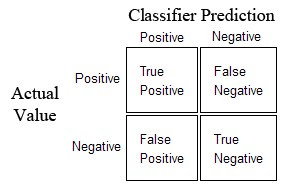
\includegraphics[width=7cm]{images/confusion_matrix.jpg}
			\end{figure} \\
			\hline
		\end{tabular}
	\end{adjustbox}
	\captionof{figure}{\textit{Confusion Matrix}}
	\label{img:confusionmatrix}
\end{table}
Contoh di atas merupakan confusion matrix untuk klasifikasi 2 kelas. Tabel memiliki 4 istilah yang akan dijelaskan sebagai berikut:

\begin{enumerate}
	\item True Positive (TP) : kondisi dimana data aktual bernilai positif dan prediksi dari klasifier bernilai positif.
	\item True Negative (TN): kondisi dimana data aktual bernilai negatif dan prediksi dari klasifier bernilai negatif.
	\item False Positive (FP): kondisi dimana data aktual bernilai negatif dan prediksi dari klasifier bernilai positif.
	\item False Negatif (FN): kondisi dimana data aktual bernilai positif dan prediksi dari klasifier bernilai negatif.
\end{enumerate}

Dari perhitungan di atas terdapat persamaan turunan lain yang bisa digunakan untuk menghitung performa dari \textit{classifier}.

\begin{enumerate}
	\item
	\textit{Accuracy}:  menghitung nilai prediksi yang benar oleh \textit{classifier}
	\begin{table}[H]
		\small
		\begin{adjustbox}{width=1\textwidth}
			\begin{tabular}{|p{13.55cm}|}
				\hline
				\begin{equation}
				Accuracy=(True Positives+True Negatives)/TotalData
				\end{equation}\\
				\hline
			\end{tabular}
		\end{adjustbox}
	\end{table}
	
	\item
	\textit{Misclassification Rate}: menghitung nilai kesalahan klasifikasi oleh \textit{classifier.} 
	\begin{table}[H]
		\small
		\begin{adjustbox}{width=1\textwidth}
			\begin{tabular}{|p{13.55cm}|}
				\hline
				\begin{equation}
				Misclassification\ Rate=(False Positives+False Negatives)/TotalData
				\end{equation}\\
				\hline
			\end{tabular}
		\end{adjustbox}
	\end{table}	
	
	\item
	\textit{True Positive Rate}: menghitung nilai prediksi bernilai positif ketika data aktual bernilai positif.
	\begin{table}[H]
		\small
		\begin{adjustbox}{width=1\textwidth}
			\begin{tabular}{|p{13.55cm}|}
				\hline
				\begin{equation}
				True \ Positive \ Rate\ (Recall)=True Positives/Actual Yes)
				\end{equation}\\
				\hline
			\end{tabular}
		\end{adjustbox}
	\end{table}
	
	\item
	\textit{False Positive Rate}: menghitung nilai prediksi positif ketika data aktual bernilai negatif.
	\begin{table}[H]
		\small
		\begin{adjustbox}{width=1\textwidth}
			\begin{tabular}{|p{13.55cm}|}
				\hline
				\begin{equation}
				False \ Positive \ Rate=False Positive/Actual No
				\end{equation}\\
				\hline
			\end{tabular}
		\end{adjustbox}
	\end{table}	
	
	\item
	\textit{Specificity}: menghitung nilai prediksi negatif ketika data aktual bernilai negatif. 
	\begin{table}[H]
		\small
		\begin{adjustbox}{width=1\textwidth}
			\begin{tabular}{|p{13.55cm}|}
				\hline
				\begin{equation}
				Specificity=True Negatives/Actual No
				\end{equation}\\
				\hline
			\end{tabular}
		\end{adjustbox}
	\end{table}
	
	\item
	\textit{Precision}: menghitung nilai prediksi positif yang benar.
	\begin{table}[H]
		\small
		\begin{adjustbox}{width=1\textwidth}
			\begin{tabular}{|p{13.55cm}|}
				\hline
				\begin{equation}
				Precision=True Positives/Predicted  Yes
				\end{equation}\\
				\hline
			\end{tabular}
		\end{adjustbox}
	\end{table}	
	
	\item
	\textit{Prevalence}: menghitung seberapa sering data aktual bernilai positif muncul.
	\begin{table}[H]
		\small
		\begin{adjustbox}{width=1\textwidth}
			\begin{tabular}{|p{13.55cm}|}
				\hline
				\begin{equation}
				Prevalence=Actual Yes/TotalData
				\end{equation}\\
				\hline
			\end{tabular}
		\end{adjustbox}
	\end{table}
	
\end{enumerate}

\subsection{Penggunaan \textit{Library}}
Berikut adalah penjelasan dari \textit{library} yang digunakan di dalam penelitian. \\
\subsubsection{OpenCV}
\textit{Library} yang digunakan adalah OpenCV untuk proses \textit{pre-processing} citra. OpenCV merupakan \textit{library open-source} yang banyak digunakan untuk penelitian terkait proses pengolahan citra dan \textit{computer vision}. 
\begin{small}
	\begin{longtable}{| p {0.5cm} | p {6cm} | p {6cm} |}
		\caption{Tabel fungsi \textit{Library} OpenCV} \\
		\hline
		\textbf{No} & \textbf{\textit{Function}} & \textbf{Deskripsi}\\
		\hline
		\endfirsthead
		
		\multicolumn{3}{c}{\textbf{\tablename~\thetable} \textit{Tabel fungsi \textit{Library} OpenCV} (Lanjutan)}\\
		\hline
		\textbf{No} & \textbf{\textit{Function}} & \textbf{Deskripsi}\\
		\endhead\noindent
		1 & Imgcodecs.imread(String filename) & Mengambil citra dari \textit{path} yang diisikan ke parameter.\\
		\hline
		2 & Imgproc.cvtColor(Mat src, Mat dst, int code) & Mengubah jenis warna pada citra sesuai yang diinginkan. Parameter fungsi ini terdiri dari Mat asal, Mat tujuan, dan \textit{code}. \textit{Code} digunakan untuk memilih tipe konversi citra tersebut, misal \textit{grayscale}.\\
		\hline
		3 & Imgproc.Canny(Mat image,Mat edges,double threshold1, double threshold2) & Fungsi ini digunakan untuk mendeteksi tepian pada citra menggunakan Canny.\\
		\hline
		4 & Imgproc.GaussianBlur(Mat src, Mat dst, Size ksize, double sigmaX) & Melakukan \textit{Gaussian Filter} terhadap citra yang dimasukkan ke dalam parameter dengan ukuran \textit{kernel} dan nilai \textit{sigma} yang diberikan.\\
		\hline
		5 & Imgproc.threshold(Mat src, Mat dst, double thresh, double maxval, int type) & Melakukan \textit{thresholding} terhadap seluruh nilai piksel dari citra yang dijadikan masukkan dengan nilai \textit{threshold}, nilai maksimum, serta jenis metode \textit{thresholding} yang digunakan, misalnya metode \textit{thresholding} Otsu.\\
		\hline
		6 & Imgproc.findContours(Mat image, List<MatOfPoint> contours, Mat hierarchy, int mode, int method) & Melakukan pencarian kontur terhadap citra yang dijadikan masukkan.\\
		\hline
		7 & Imgproc.contourArea(Mat contour) & Melakukan perhitungan luas area dari kontur yang diberikan.\\
		\hline
		8 & Imgproc.imwrite(String filename, Mat img) & Menyimpan citra yang diisikan ke parameter ke \textit{path} yang dijadikan tujuan penyimpanan.\\
		\hline
	\end{longtable}
\end{small}

\section{Tinjauan Studi}
Terdapat beberapa metode yang dapat digunakan untuk melakukan deteksi mobil pada citra digital. Tabel 2.1 akan menjelaskan tentang metode-metode tersebut beserta hasil dari
penerapannya.
\begin{small}
	\begin{longtable}{| p {0.5cm} | p {3cm} | p {3.5cm} | p {3.5cm} | p {3.5cm} |}
		\caption{Tabel Tinjauan Studi} \\
		\hline
		\textbf{No}  & \textbf{Judul}  & \textbf{Masalah}  & \textbf{Metode}  & \textbf{Hasil} \\
		\hline
		\endfirsthead
		\hline
		\textbf{No}  & \textbf{Judul}  & \textbf{Masalah}  & \textbf{Metode}  & \textbf{Hasil} \\
		\hline
		\endhead
		1  & Adhi Prahara, Murinto "Car Detection Based on Road Direction on Traffic		Surveillance Image" & Mendeteksi mobil dari semua sudut pandang kamera pengawas. & HOG, SVM & Area jalan diekstraksi untuk menentukan area deteksi dan arah jalanan digunakan untuk menentukan detektor mobil yang akan digunakan oleh Linear-Support Vector Machine (Linear-SVM). \\
		\hline
		2  & Daniel Neumann, Tobias Langner, Fritz Ulbrich, Dorothee Spitta1and Daniel Goehring "Online  Vehicle  Detection  using  Haar-like,  LBP  and  HOG  Feature  basedImage  Classifiers  with  Stereo  Vision  Preselection" & Membandingkan metode ekstraksi fitur. & Haar-like, LBP, dan HOG & Memberikan perbandingan penggunaan metode ekstraksi fitur antara Haar-like, LBP, dan HOG. \\
		\hline
		3  & A.Shakin Banu dan P. Vasuki "Video Based Vehicle Detection Using Morphological Operation and HOG Feature Extraction" & Penggunaan proses morfologi dan HOG untuk mendeteksi objek. & Morphological Operation, HOG & Hasil analisis menerangkan bahwa deteksi kendaraan menggunakan metode ini mencapai tingkat kesuksesan dengan akurasi sekitar 83 persen. \\
		\hline
		4  & G. Adhika dan R.R.W. Ken "Penerapan Histogram of Oriented Gradients, Principal Component Analysis, dan AdaBoost untuk Sistem Pengenalan Wajah" & Penggunaan proses HOG, PCA, dan AdaBoost untuk pengenalan wajah. & HOG, PCA, AdaBoost & Hasil analisis menerangkan bahwa pengenalan wajah menggunakan metode PCA dapat meningkatkan akurasi. \\
		\hline
	\end{longtable}
\end{small}

Pada penelitian yang dilakukan Adhi Prahara et al., mengusulkan framework dengan metode HOG dan SVM untuk mendeteksi mobil. Pertama, dataset dibagi menjadi data latih dan data uji. Data dikelompokkan berdasarkan sudut pandang (depan atau belakang, kiri atas atau kanan bawah, kanan atas atau kiri bawah, kiri atau kanan). Selanjutnya, untuk menentukan sudut pandang, dilakukan deteksi arah jalan. Terakhir, metode HOG dan SVM digunakan untuk deteksi mobil.

Pada penelitian yang dilakukan Daniel Neumann et al., menerapkan detektor DPM (DeformableParts Model), di mana bagian-bagian dari pola gambar dilatih dengan peningkatan resolusi oleh filter bagian. Untuk dapat mengidentifikasi kendaraan digunakan klasifikasi gambar dan melatihnya pada tampilan belakang kendaraan. Kemudian menerapkan berbagai algoritma \textit{computer vision} yang efisien.

Pada penelitian yang dilakukan A. Shakin Banu et al., mengusulkan framework dengan metode morphological operations dan HOG untuk mendeteksi mobil. Pertama, akan dilakukan pemilihan ROI (\textit{Region of Interest}) untuk mengurangi penggunaan memori. Berdasarkan hasil pre-procesing, citra akan diterapkan Sobel edge Detection sehingga didapatkan fitur gradien fungsi intensitas dari frame yang kemudian digunakan untuk perhitungan gradien. Terakhir, metode morphological operation akan dilakukan untuk menghapus objek yang tidak seharusnya terdeteksi, sehingga mengurangi piksel dalam frame. HOG kemudian diterapkan untuk ekstraksi fitur dan SVM untuk menentukan apakah mobil atau bukan.

Pada penelitian yang dilakukan G. Adhika et al., menjelaskan bahwa terdapat banyak faktor yang mempengaruhi hasil pengenalan seperti kualitas citra, ekspresi wajah dan kemiripan bentuk dari komponen wajah manusia dimana hal tersebut mempengaruhi fitur HOG yang dihasilkan. Penggunaan metode PCA meningkatkan akurasi dari HOG dan AdaBoost dari 86\% menjadi 96\% dengan ukuran sel sebesar 8, blok sebesar 16, dan bin sebesar 16.\\

\section{Tinjauan Objek}
Pada bagian ini akan dijelaskan mengenai objek terkait yang akan digunakan dalam
penelitian ini.\\

\subsection{Deteksi Mobil}
Mobil adalah kendaraan darat yang digerakkan oleh tenaga mesin, beroda empat atau lebih (selalu genap), biasanya menggunakan bahan bakar minyak (bensin atau solar) untuk menghidupkan mesinnya. Jenis mobil yang terdeteksi terdiri 3 golongan yaitu kendaraan kecil, kendaraan sedang, dan kendaraan besar.  Hasil yang diperoleh dapat dimanfaatkan untuk mengetahui lokasi kendaraan yang melewati jalan tersebut dalam suatu interval waktu tertentu. Citra mobil yang digunakan merupakan hasil citra dari sudut horizontal yang diambil dari dasbor mobil. Contoh citra mobil dan hasil visualisasi fitur HOG dapat dilihat pada gambar \ref{img:car}.
\begin{table}[H]
	\small
	\begin{adjustbox}{width=1\textwidth}
		\begin{tabular}{| p {14cm} |}
			\hline
			\begin{figure}[H]
				\centering
				\subfloat[ ]{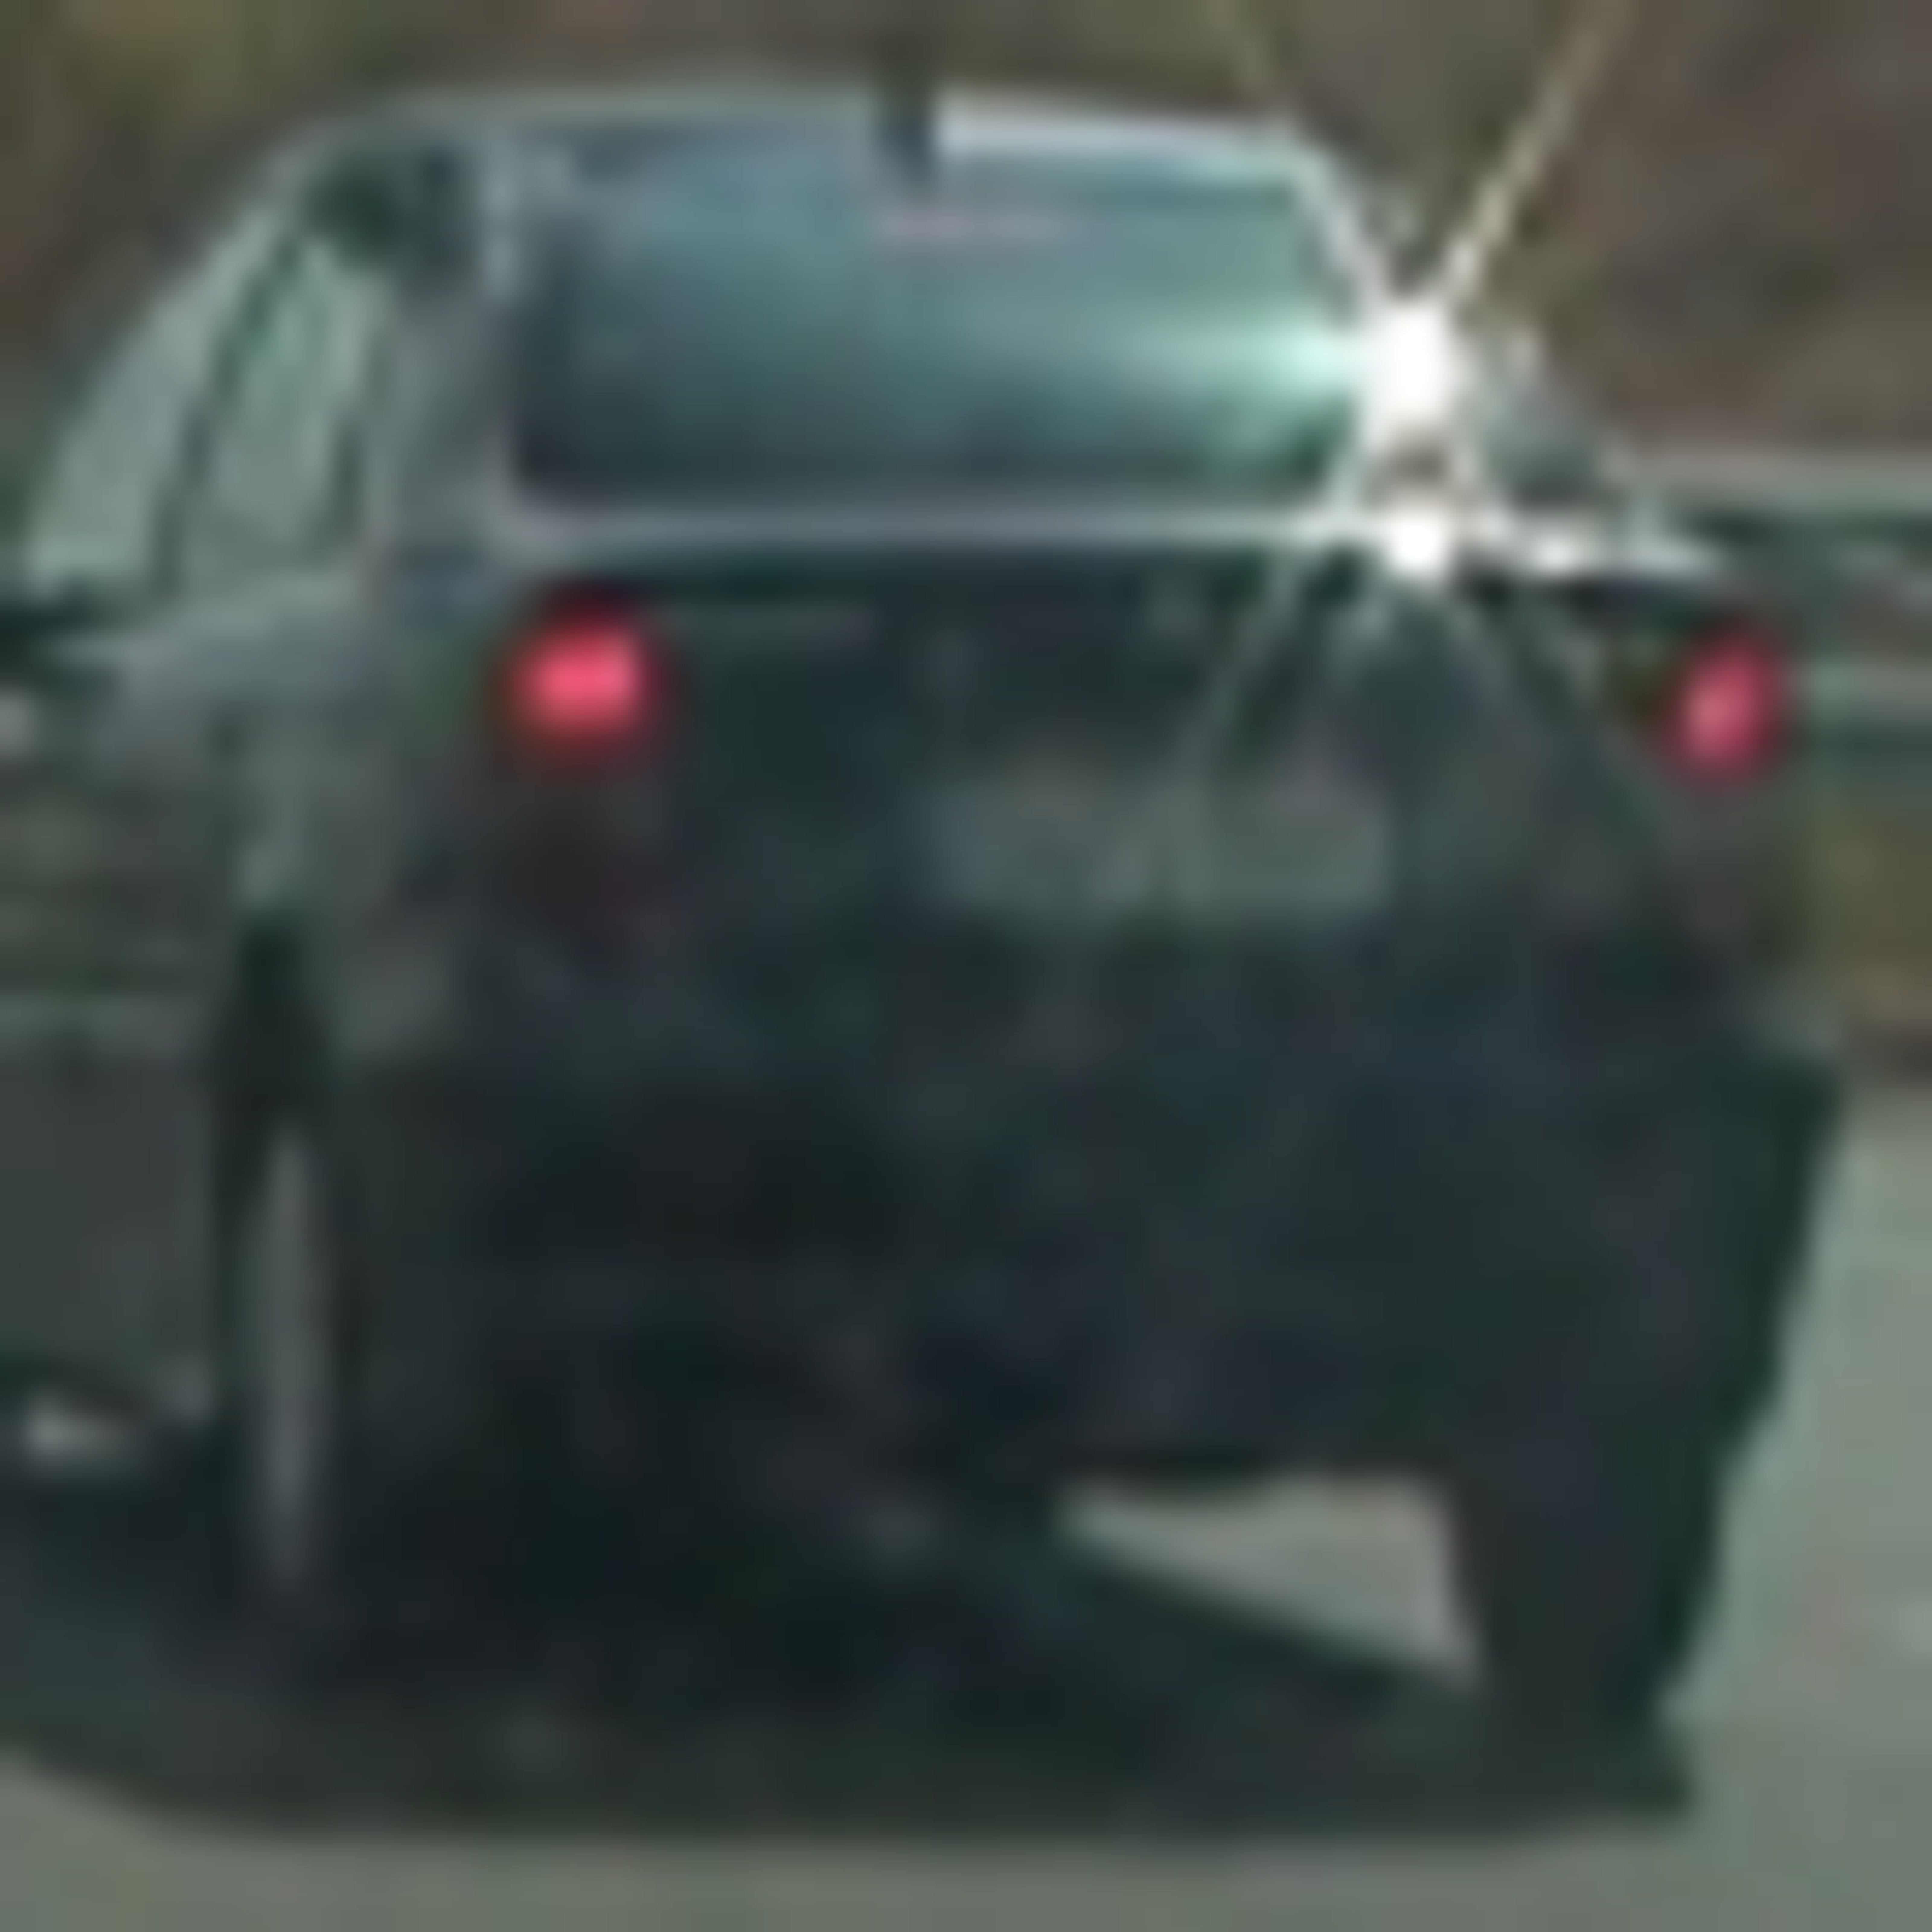
\includegraphics[width=7cm]{images/car.png}}
				\subfloat[ ]{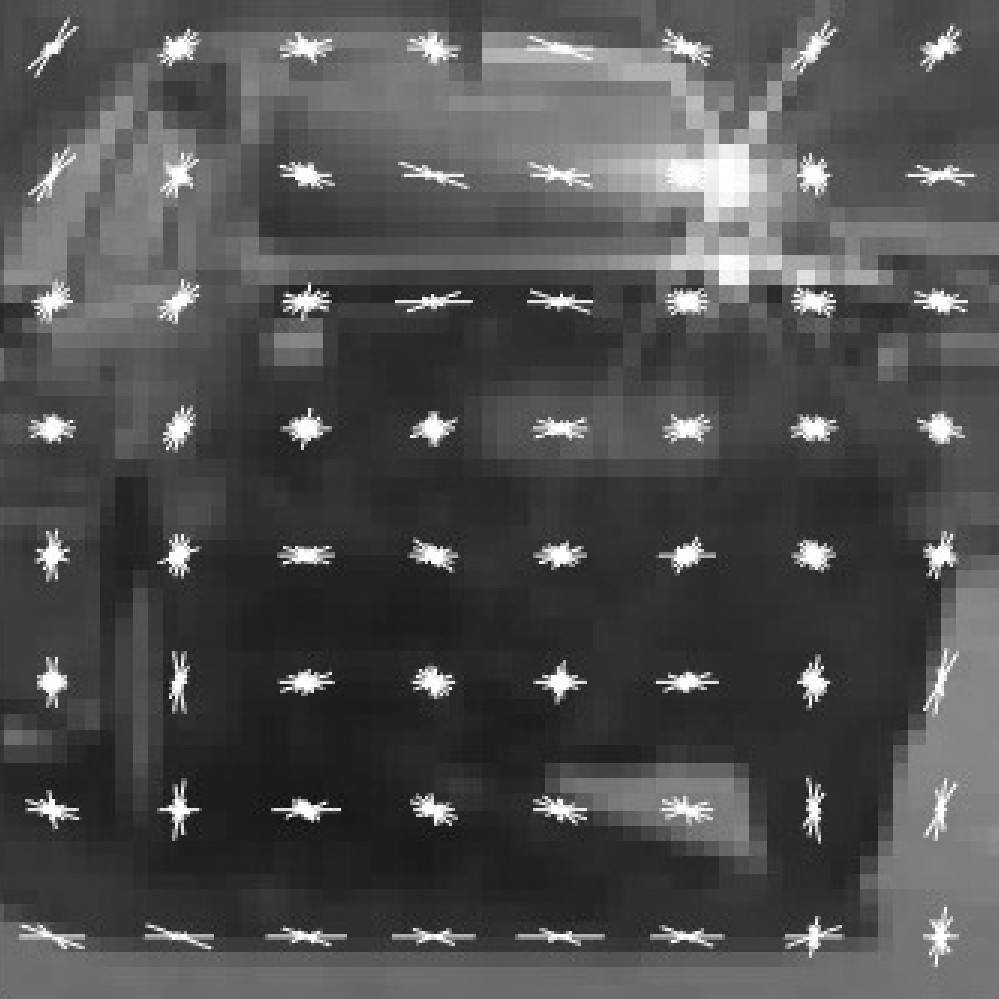
\includegraphics[width=7cm]{images/car_hog_gray8x8.jpg}}
			\end{figure} \\
			\hline
		\end{tabular}
	\end{adjustbox}
	\captionof{figure}{Citra Mobil nampak dari belakang. (a) Citra masukkan (b) Visualisasi fitur HOG}
	\label{img:car}
\end{table}
\newpage